\chapter{Newtonian elastic-plated gravity current} 
\label{chap2} 
\minitoc

In this chapter, we  sum up the main tentative that  have been used to
describe the emplacement of magmatic intrusions in the upper crust.

\section{Theoretical model}
\label{C2-sec:model}

At shallow  depth in  the upper  crust, roof  lifting is  the dominant
process     by    which     magma     makes     room    for     itself
\citep{Johnson:1973ho,Pollard:1973ho}, which leads  to the deformation
and bending of the overlying  strata.  Such system is commonly modeled
as an  isoviscous elastic-plated gravity current,  i.e.  an isoviscous
fluid spreading  beneath a thin  elastic sheet of thickness  $d_c$ and
above  a  rigid   layer  \citep{Michaut:2011kg,Bunger:2011cb}  (Figure
\ref{C2-Sketch}).  The  behavior of isoviscous  elastic-plated gravity
current have  been largely  discussed in  the past  few years  in both
carthesian \citep{Michaut:2011kg,Bunger:2011cb,Anonymous:QWXp_4JV} and
axisymmetrical  geometry  \citep{Michaut:2013dr,Lister:2013ia}.   This
section details  a summary of the  results for an isoviscous  fluid of
density $\rho_m$ and  viscosity $\eta$, supplied at  a continuous rate
$Q(t)$ through a cylindrical conduit of  diameter $a$ at the center, in
an axisymmetrical  geometry (Figure \ref{C2-Sketch}). This  model will
constitute the reference for more elaborate models in the manuscript.

\begin{figure}[htbp]
  \begin{center}
    \graphicspath{ {/Users/thorey/Documents/These/Manuscript/Figure/Chapter2/} }
    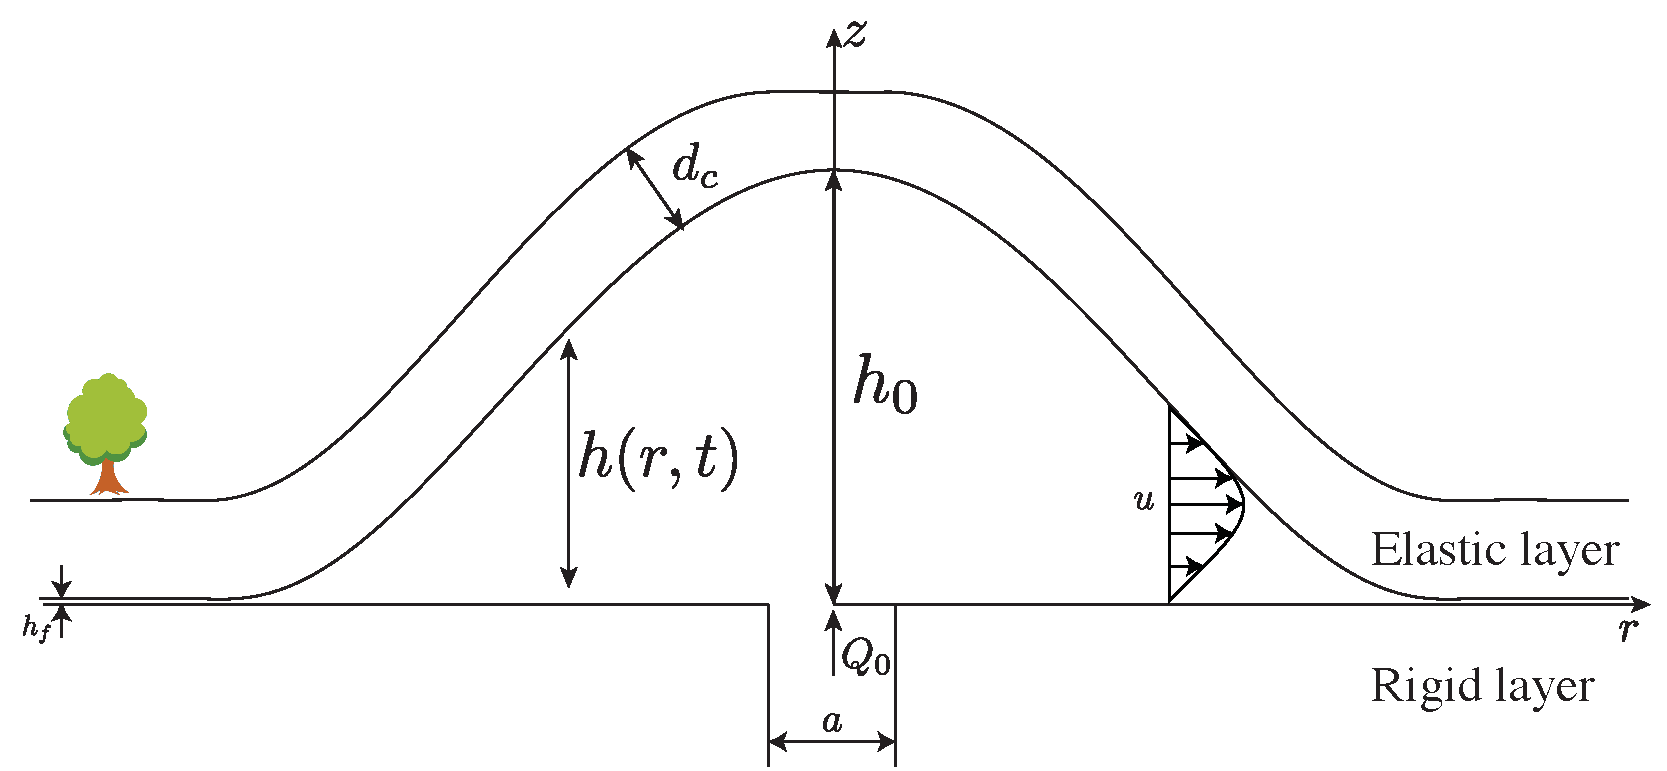
\includegraphics[scale=0.40]{C2_Sketch.pdf}
    \caption{Model geometry and parameters.}
    \label{C2-Sketch}
  \end{center}
\end{figure}

\subsection{Governing equation}
\label{C2-sec:Governing equation}

\textbf{Driving pressure}\\

The  intrusion develops  over a  length scale  $\Lambda$ that  is much
larger than its thickness $H$ ($\Lambda >> H$).  In the laminar regime
and  in   axisymmetrical  coordinates  ($r$,$z$),   the  Navier-stokes
equations within the lubrication assumption are
\begin{eqnarray}
  -\frac{\partial P}{\partial r}  +  \frac{\partial}{\partial z}\left(\eta \frac{\partial u}{\partial z}\right) &=&0\label{C2_V1} \\
  -\frac{\partial P}{\partial z}  - \rho_{m}g&  =&0\label{C2-Npressure}
\end{eqnarray}
where  $u(r,z,t)$  is  the  radial   velocity,  $g$  is  the  standard
acceleration due to gravity and  $P(r,z,t)$ is the pressure within the
fluid.   Integration  of  (\ref{C2-Npressure}) thus  gives  the  total
pressure  $P(r,z,t)$ within  the flow.   When the  vertical deflection
deflection $h(r,t)$  of the upper  elastic layer is small  compared to
its thickness  $d_c$, i.e $h<<d_c$,  we can neglect stretching  of the
upper layer and only consider  bending stresses.  Therefore, the total
pressure $P(r,z,t)$ at a level $z$ in the intrusion is the sum of four
contributions: the  weight of the  magma and  of the upper  layer, the
bending pressure $P_b$ and the atmospheric pressure $P_0$
\begin{equation}
  P = \rho_m g (h-z)+\rho_rgd_c+P_b+P_0
  \label{C2-pression}
\end{equation}
where $h(r,t)$ is the intrusion  thickness and $\rho_r$ the density of
the surrounding rocks. The bending pressure  is given by the force per
unit area  that is necessary  for a  vertical displacement $h$  of the
thin elastic plate \citep{Turcotte:1982ca}
\begin{equation}
  P_d = D\nabla^4h
\end{equation}
where $D$  is the flexural  rigidity of  the thin elastic  layer, that
depends on the Young's modulus $E$, Poisson's ratio $\nu^*$ and on the
elastic           layer          thickness           $d_c$          as
$D = Ed_c^3/\left(12(1-\nu^*)\right)$.

\vspace{.5cm} \textbf{Velocity field} \vspace{.5cm}

Equation (\ref{C2_V1})  can be integrated  twice as a function  of $z$
using the boundary conditions
\begin{eqnarray}
  u(r,0,t) &=& 0 \hspace{.5cm} \text{No-slip boundary condition}\\
  u(r,h(r,t),t) &=& 0 \hspace{.5cm} \text{No-slip boundary condition}
\end{eqnarray}
leading to the expression of the horizontal velocity
\begin{equation}
  u(r,z,t) =\frac{1}{2\eta} \frac{\partial P}{\partial r} \left(z^2-hz\right)
  \label{C2-deriv}
\end{equation}

\vspace{.5cm} \textbf{Injection rate} \vspace{.5cm}

The effective overpressure $\Delta P^*$ driving the flow in the feeder
conduit decreases as the intrusion thickens and is given by
\begin{equation}
  \Delta P^* = \Delta P -\rho_m g h_0 \label{C2-Q0}
\end{equation}
where $h_0(t)$ is the maximum  intrusion thickness at the center $r=0$
and $\Delta P$ is the initial  driving pressure or the overpressure at
the base of the dyke ($z = -Z_c$).

In (\ref{C2-Q0}), the bending pressure  at then center, which scale as
D$h_0(t)/R(t)^4$  where  $R(t)$  is   the  blister  radius,  has  been
neglected.  Although  it tends  to infinity at  the initiation  of the
flow, it rapidly  vanishes as the blister spreads  and the hydrostatic
pressure $\rho_m g h_0$ becomes  the main contribution to the pressure
at the  center.  In addition, the  model assumes a large  aspect ratio
for the blister and does not consider the initiation of the flow.

Finally,  assuming a  Poiseuille flow  within the  cylindrical feeding
conduit, the vertical injection velocity $w_i(r,t)$ and injection rate
$Q(t)$ are given by
\begin{equation}
  w_i=
  \begin{cases}
    \frac{ \Delta P^*}{4 \mu Z_{c}} (\frac{a^{2}}{4}-r^{2})& r \le \frac{a}{2}\\
    0 & r > \frac{a}{2}
  \end{cases}
  \label{C2-eq12}
\end{equation}
\begin{equation}
  Q = Q_0(1-\frac{\rho_m g h_0}{\Delta P})
  \label{C2-eq11}
\end{equation}
where
$Q_0=\left(\pi \Delta P^* a^{4}\right)/\left(128 \eta Z_c\right)$.

\vspace{.5cm} \textbf{Mass conservation} \vspace{.5cm}

The fluid  is assumed  incompressible and a  global statement  of mass
conservation gives
\begin{eqnarray}
  \frac{\partial         h}{\partial        t} +\frac{1}{r}
  \frac{\partial}{\partial
  r} \left( r\int_0^hudz\right) = w_i.
  \label{C2-Mass}
\end{eqnarray}
which can be rewrite as
\begin{eqnarray}
  \frac{\partial         h}{\partial        t} -\frac{1}{r}
  \frac{\partial}{\partial
  r} \left( r\int_0^h\frac{\partial u}{\partial z}zdz\right) = w_i
  \label{C2-Mass-2}
\end{eqnarray}
where we  used no slip-boundary conditions  at the top and  the bottom
$u(r,z=h,t)=u(r,z=0,t)=0$.   The integration  of (\ref{C2_V1}),  using
$\left.\frac{\partial  u}{\partial  z}\right|_{z=h/2}=0$ by  symmetry,
gives
\begin{equation}
  \frac{\partial     u}{\partial    z}=     \frac{1}{\eta}\frac{\partial
    P}{\partial r} \left(z-\frac{h}{2}\right).
  \label{C2-deriv}
\end{equation}
and therefore, injecting (\ref{C2-deriv})  and substituting $P$ by its
expression (\ref{C2-pression}) in (\ref{C2-Mass-2}) finally gives
\begin{equation}
  \frac{\partial h}{\partial t} = \frac{1}{r}
  \frac{\partial}{\partial r} \left( r\left(\rho_m g \frac{\partial h}{\partial      r}+D\frac{\partial}{\partial      r}\left(\nabla^4h\right)\right)I\right)
  + w_i.
  \label{C2-EqConservation}
\end{equation}
where
\begin{equation}
  I = \int_0^h\frac{1}{\eta}\left(z-\frac{h}{2}\right)z dz
  \label{C2-Integral}
\end{equation}
depends on the considered rheology. In the case of an isoviscous flow,
the integral in (\ref{C2-Integral}) is easily derived and the equation
becomes
\begin{equation}
  \frac{\partial h}{\partial t} =\frac{\rho_mg}{12 \eta r}
  \frac{\partial}{\partial r}  \left( rh^3  \frac{\partial h}{\partial
      r}\right)+\frac{D}{12\eta r} \left( rh^3 \frac{\partial}{\partial r}\nabla^4h\right)+
  w_i .\label{C2-Heq}
\end{equation}

The evolution equation for  the flow thickness $h(r,t)$ (\ref{C2-Heq})
is composed of three different terms on the right hand side. The first
term  represents  gravitational  spreading,  i.e.   spreading  of  the
blister under its own weight. The second term represents the squeezing
of the  flow by the upper  elastic layer.  Both term  are negative and
induces spreading.   The last term  represents fluid injection  and is
positive.

\subsection{Dimensionless equations}
\label{C2-sec:dimens-equat}

Equations  (\ref{C2-eq12}) and  (\ref{C2-Heq}) are  nondimensionalized
using a  horizontal scale $\Lambda$, a  vertical scale $H$ and  a time
scale $\tau$ given by
\begin{eqnarray}
  \Lambda &=& \left(\frac{D}{\rho_m g}\right)^{1/4}\label{L1}\\
  H&=&\left       (\frac{12\eta      Q_{0}}{\rho_{m}g       \pi}\right      )
       ^{\frac{1}{4}} \label{H1}\\
  \tau&=&\frac{\pi \Lambda^{2} H}{Q_{0}}\label{T1}
\end{eqnarray}

where scales  are chosen  such that $Q_0  = \pi\Lambda^2  H/\tau$. The
length scale $\Lamba$ represents the  flexural wavelength of the upper
elastic layer,  i.e. the  length scale at  which bending  stresses and
gravity  contributes equally  to flow.   The height  scale $H$  is the
thickness of  a typical gravity current  and the time scale  $\tau$ is
the  characteristic time  to  fill  up a  cylindrical  flow of  radius
$\Lambda$ and thickness  $H$ at constant rate $Q_0$.   In addition, we
can       define        a       horizontal        velocity       scale
$U=\Lambda/\tau=\left(\rho_m           g           H^3\right)/\left(12
  \eta_h\Lambda\right)$.

The dimensionless equation is
\begin{eqnarray}
  \frac{\partial h}{\partial t}& =&\frac{1}{ r}
                                    \frac{\partial}{\partial r}  \left( rh^3  \frac{\partial h}{\partial
                                    r}\right)+\frac{1}{ r} \left( rh^3 \frac{\partial}{\partial r}\nabla^4h\right)+
                                    \frac{32}{\gamma^{2}}\left(\frac{1}{4}-\frac{r^{2}}{\gamma^{2}}\right)\left(1-\frac{h_0}{\sigma}\right)
\end{eqnarray}
where the last term is replaced by zero for $r<\gamma/2$.

$\gamma$ and $\sigma$  are two dimensionless numbers  that control the
dynamics of the flow
\begin{eqnarray}
  \gamma &=& \frac{a}{\Lambda}\\
  \sigma &=& \frac{\Delta P}{\rho_m g h}.
\end{eqnarray}
$\gamma$  is the  dimensionless radius  of  the conduit,  it does  not
significantly influence the flow and is set to $0.02$ in the following
\citep{Michaut:2009jx,Michaut:2011kg}.   $\sigma$  is  the  normalized
pressure  head,  i.e.,  the  ratio between  the  initial  overpressure
driving the flow and the weight of the magma at the center.
	 
\subsection{Need for regularization}
\label{C2-sec:need-regularization}


\section{Regime of propagations}
\label{C2-sec:regime-propagations}

The dynamics show three main spreading regime.

\subsection{Bending regime}
\label{C2-sec:bending-regime}

\subsection{Gravity current regime}
\label{C2-sec:grav-curr-regime}


  For a constant  injection rate, a small  pre-wetting film thickness,
  i.e.   $h_f/H<<1$  and   a  viscosity  contrast  $\nu$   set  to  1,
  $\int_0^h u  dz=-h^3 \frac{\partial  P}{\partial r}$,  the numerical
  resolution  of the  equation  (\ref{EqFinal1})  shows two  spreading
  regimes    \citep{Michaut:2011kg,Bunger:2011cb,Lister:2013ia}.    At
  early  times,  when  $R<<\Lambda$,  gravity is  negligible  and  the
  dynamics of  the spreading is governed  by the bending of  the upper
  layer.   The spreading  is very  slow and  the interior  has uniform
  pressure $P =\nabla^4h$.  The flow  is bell-shaped and its thickness
  is given by
  \begin{equation}
    h(r,t) = h_0(t)\left(1-\frac{r^2}{R^2(t)}\right)^2
    \label{IntrusionShape}
  \end{equation}
  with  $h_0(t)$  the  thickness  of   the  intrusion  at  the  center
  \citep{Michaut:2011kg,Lister:2013ia}.       In     this      regime,
  \citet{Lister:2013ia} have shown that the spreading is controlled by
  the propagation of a peeling by  bending wave at the intrusion front
  with dimensionless velocity $c$
  \begin{equation}
    c=    \frac{\partial             R}{\partial            t}             =h_f^{1/2}
    \left(\frac{\kappa}{1.35}\right)^{5/2}
    \label{WaveVelocity}
  \end{equation}
  where  $\kappa =  \partial^2  h/\partial r^2$  is the  dimensionless
  curvature  of  the interior  solution.   Using  the propagation  law
  (\ref{WaveVelocity})  and   the  form   of  the   interior  solution
  (\ref{IntrusionShape}), they find that the  radius and the height of
  the intrusion are given by similarity solutions
  \begin{eqnarray}
    R(t) &=& 2.2h_f^{1/22}t^{7/22}\label{ScalingR}\\
    h_0(t)&=&0.67 h_f^{-1/11}t^{8/22}\label{ScalingH}.
  \end{eqnarray}
  where the numerical pre-factor have been matched to our simulations.
  In addition,  the peeling  length scale  $L_p$ at  the front  can be
  quantified in term  of the local wave velocity  and fluid parameters
  and follow in a dimensionless form
  \begin{equation}
    L_p(t) &=&1.07h_f^{13/22}t^{3/22}.
    \label{Lp}
  \end{equation}
  In  contrast,  when  the  radius R  becomes  larger  than  $\Lambda$
  ($R>>\Lambda$), the  weight of  the intrusion becomes  dominant over
  the  bending  terms.   The  pressure is  given  by  the  hydrostatic
  pressure  $P =  h$  and  the intrusion  enters  a classical  gravity
  current regime where bending terms only affect the solution near the
  intrusion  edge  \citep{Huppert:1982a,Michaut:2011kg,Lister:2013ia}.
  In  this second  regime, the  radius  evolves as  $t^{1/2}$ and  the
  thickness tends to a constant
  \begin{eqnarray}
    R(t) &=& 0.715 t^{1/2}\label{Scaling-R-Gravi}\\
    h_0 &=& 1.86\label{Scaling-H-Gravi}
  \end{eqnarray} 
  In the following, we study the  effect of the cooling on the blister
  dynamics in  both regime  separately for  a constant  film thickness
  $h_f=5\cdot10^{-3}$.

\section{Application to the Earth, Moon and Mars}
\label{C2-sec:appl-earth-moon}

\section{Discussion}
\label{C2-sec:discussion}

\begin{table}
  \caption{Range of values for the model parameters}
  \centering
  \begin{tabular}{c|c|c|c}
    \hline
    Parameters& Symbol & Range of values &Unit\\
    \hline
              &&\\
    Depth of intrusion & $d_c$ & $0.1-5$ &km \\
    Young's Modulus & $E$ & $10-100$ &GPa \\
    Poisson's ratio & $\nu^*$ & $0.25$ &\\
    Gravity & $g$ & $9.81$ &m s$^{-2}$ \\
    Magma density & $\rho_{m}$ & $2800-3200$ &kg m$^{-3}$ \\
    Magma viscosity & $\eta $ & $1-10^{4}$ &Pa s \\
    Feeder dyke width & $a$ & $1-100$ &m \\
    Depth of the melt source & $Z_{c}$ & $ 5-500$& km \\ 
    Initial overpressure & $\Delta P$ & $5-50$ &MPa \\
    Injection rate & $Q_{0}$ &$10p{-3}-0.1$ &m$^{3}$ s$^{-1}$ \\
    Crust density & $\rho_{r}$ & $2500$ &kg m$^{-3}$ \\
              &&\\
    \hline
    Characteristic scales & Symbol & Range of values & Unit\\
    \hline
              &&\\
    Height scale & $H$& $0.1-10$ &m \\
    Length scale & $\Lambda$ & $1-12$& km \\
    Time scale & $\tau$ & $10^{-1}-10$ &years \\
                                              \label{tab2}
  \end{tabular} 
\end{table}
\begin{table}
  \caption{Dimensionless numbers}
  \centering
  \begin{tabular}{c|c|c|c}
    &&Complex craters&Simple craters \\
    \hline
    Symbol& Description & Range of values & Range of values \\
    \hline
    &&\\
    $\gamma$&Normalized source width& $10^{-4}-10^{-2}$ &$10^{-4}-10^{-2}$ \\
    $\zeta$& Normalized wall zone width  & $0.05-0.13$&$0.25$\\
    $\Psi$&Thickening term & $0.3-8$&$0.2-4$\\
    $\Xi$& Hydrostatic term & $20-400$&$20-200$\\
    $\Theta$ &Elastic term & $10^{-7}-0.1$&$10^{-3}-10$\\
    $\Omega$ & Density ratio & $1.2$ &$1.2$\\
    $\Phi$ & Upper layer aspect ratio & $4500$ &$1200 $\\
    $\sigma$&Normalized pressure head& $0.6-100$ & $0.6-100$ 
                                                   \label{tab3}
  \end{tabular} 
  % \tablenotetext{a}{Footnote text here.}
\end{table}
%%% Local Variables:
%%% mode: latex
%%% TeX-master: "../main"
%%% End:
